%%%%%%%% ICML 2021 EXAMPLE LATEX SUBMISSION FILE %%%%%%%%%%%%%%%%%

\documentclass{article}

% Recommended, but optional, packages for figures and better typesetting:
\usepackage{microtype}
\usepackage{graphicx}
\usepackage{subfigure}
\usepackage{booktabs} % for professional tables

% hyperref makes hyperlinks in the resulting PDF.
% If your build breaks (sometimes temporarily if a hyperlink spans a page)
% please comment out the following usepackage line and replace
% \usepackage{icml2021} with \usepackage[nohyperref]{icml2021} above.
\usepackage{hyperref}

% Attempt to make hyperref and algorithmic work together better:
\newcommand{\theHalgorithm}{\arabic{algorithm}}

% Use the following line for the initial blind version submitted for review:
\usepackage[accepted]{icml2021}

% If accepted, instead use the following line for the camera-ready submission:
%\usepackage[accepted]{icml2021}

% The \icmltitle you define below is probably too long as a header.
% Therefore, a short form for the running title is supplied here:
\icmltitlerunning{Spam Detection Using Machine Learning Algorithms}

\begin{document}

\twocolumn[
\icmltitle{Spam Detection Using Machine Learning Algorithms}

% It is OKAY to include author information, even for blind
% submissions: the style file will automatically remove it for you
% unless you've provided the [accepted] option to the icml2021
% package.

\begin{icmlauthorlist}
\icmlauthor{Lucy Ren}{}
\icmlauthor{Valerie Shoemaker}{}
\end{icmlauthorlist}

% You may provide any keywords that you
% find helpful for describing your paper; these are used to populate
% the "keywords" metadata in the PDF but will not be shown in the document
\icmlkeywords{Machine Learning}

\vskip 0.5in
]

\section{Introduction}
\large
Spam has been a pervasive and deeply entrenched problem since the creation of the internet. Modern-day spam takes many forms, from SMS messages to emails, flooding inboxes with unwanted information. Spam is often used to cast a wide net and get unaware users to fall for scams and download viruses that could cause serious damage. Most modern day email clients employ many types of spam prevention measures; sorting, hiding, and deleting unwelcome mail. Our final project attempts to use machine learning techniques, including logistic regressions and SVC, in order to detect spam in our data set.

\section{Related Work}

Machine learning has become the standard method for modern email spam filters. Traditionally, spam filters made use of much simpler metrics for removing unwanted messages. Older filters made use of basic keyword and special character recognition, moving any email that violated the filters restrictions to the spam folder \cite{nlm}. ISPs also began adding email addresses and IP addresses that were known for sending spam messages to blacklists that were put in place for most clients \cite{emarsys}.

More modern approaches to filtering out spam messages have prominently featured machine learning. Using Natural Language Processing various classification models have come to the forefront of spam detection, including Naive Bayes, decision trees, and random forest algorithms \cite{hindawi}. Much more recently, some studies have attempted to use pre-trained Bidirectional Encoder Representations from Transformers, which have the capability to take the context of the text into account while processing, to more effectively remove spam \cite{sciencedirect}. Studies have also speculated on using Big Data analytics to better determine spam without the use of pre-trained models and pre-labeled and organized data like typical machine learning approaches \cite{springer}.

\section{Preprocessing Data}

\begin{figure}[ht]
\vskip 0.2in
\begin{center}
\centerline{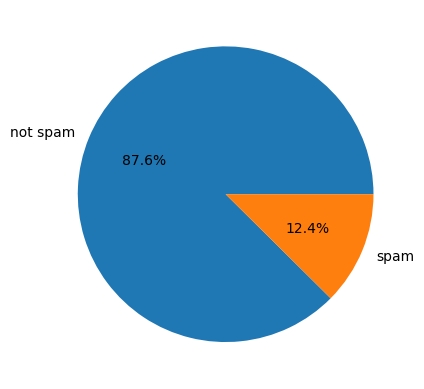
\includegraphics[width=\columnwidth]{images/image4.png}}
\caption{Pie chart of the composition of the data set.}
\end{center}
\vskip -.2in
\end{figure}

In order to make the data set easier to understand, we first converted the category column of the data set so that instead of labeling messages as “spam” or “ham” they were labeled numerically; 0 for real messages and 1 for spam messages. Next we used various text cleaning methods to make the data set easier for the models to learn from. After examining the data set we found that:

\begin{figure*}[t]
\vskip 0.2in
\centerline{
    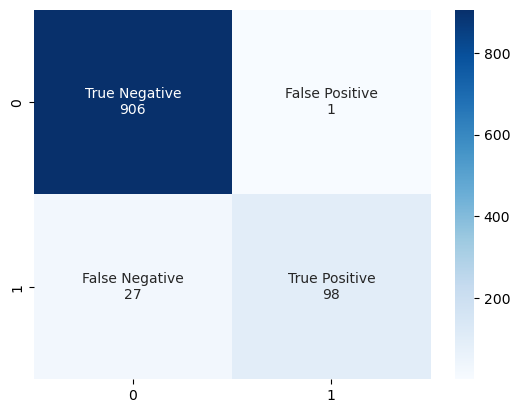
\includegraphics[width=.33\textwidth]{images/linearconfusionmatrix.png}
    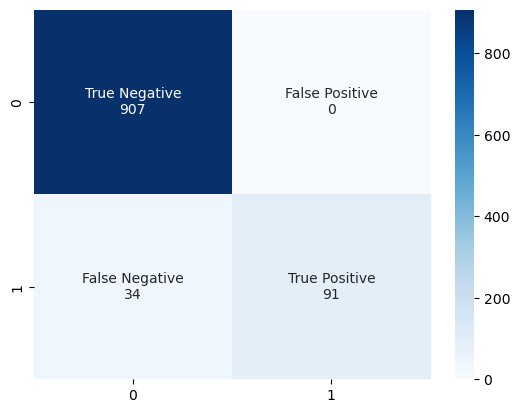
\includegraphics[width=.33\textwidth]{images/svmconfusionmatrix.png}
    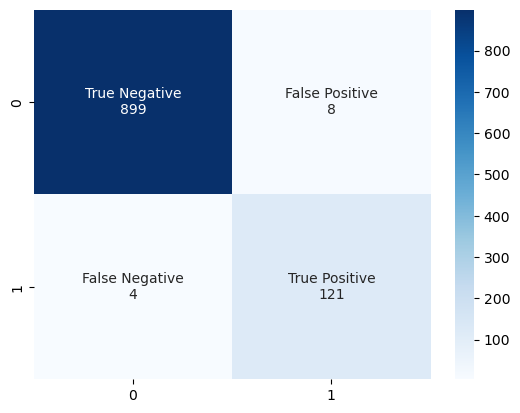
\includegraphics[width=.33\textwidth]{images/naivebayesconfusionmatrix.png}
}
\caption{Confusion matrices for Logistic Regression, SVM, and Naive Bayes models respectively.}
\vskip 0in
\end{figure*}

\begin{itemize}
\item There were multiple duplicate messages within the data set. Before we ran our models, we thought it would be best to remove all duplicate messages from the data.
\item There were many types of insignificant data within the data set, mainly stop words. We removed the stop words in order to improve the effectiveness of our models.
\item There were many phone numbers and hyperlinks within the data set. While many data sets require these to be removed in preprocessing, we decided to leave them in as they worked as a good indicator of spam messages (spam is much more likely to include links and phone numbers to scam users).
\end{itemize}

\section{Data Analysis}

\begin{figure}[ht]
\vskip 0.2in
\begin{center}
\centerline{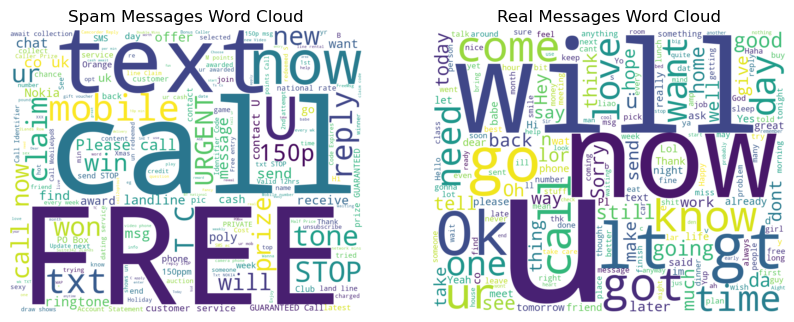
\includegraphics[width=\columnwidth]{images/wordcloud.png}}
\caption{Word clouds of words used in spam messages and real messages within the data set.}
\end{center}
\vskip -.2in
\end{figure}

The data set utilized consists of 5572 messages that have each been categorized as either spam or ham. Ham messages are considered legitimate messages. Once duplicates are removed from this data set, the number of messages drops to 5157. Within the data set, roughly 88\% of the messages have been categorized as not spam while 12\% of the messages are considered to be spam. 

The spam messages within the data set seem to use more active words such as call, text, reply, and claim, as well as references to the medium that is being used to send the message such as mobile, email, phone, and landline. While some words can be seen as fitting more clearly into one classification or the other, it's important to utilize machine learning to solve this problem as some words are used extremely frequently in both real and spam messages.

The data set was found on Kaggle and was created by Faisal Quereshi as a public data set \cite{dataset}.

\section{Models}
\subsection{Training and Testing Data}

To generate our training and testing data, we utilized the data set with only unique messages and randomly selected 80\% of the data to be training data. The remaining 20\% of the data was used as testing data. The training data included 4125 entries while the testing data included 1032 entries. 

\subsection{Logistic Regression}
Logistic Regression classification models are used when the classification target is categorical, which works well for our use case of fitting messages into categories of spam or real. Logistic Regression works by fitting the model to a sigmoid curve and matching inputs across the curve to targets around 1 or 0. 

After running the Logistic Regression classifier on our testing data, we had an accuracy of 97.29\%, precision of 98.99\%, recall of 78.4\%, and F1 score of 87.5\%.

\subsection{SVM}
Support Vector Machine models, or SVM, is widely used in both classification and regression. In our case the SVM algorithm attempts to draw a hyperplane between the two types of data with the maximum margin between sets of data.

After running the SVM classifier on our testing data, we had an accuracy of 96.71\%, precision of 100\%, recall of 72.8\%, and F1 score of 84.26\%.

\subsection{Naive Bayes}
Naive Bayes models are based on Bayes’ Theorem, which gives the compound probability of two independent events. Because Naive Bayes models assume that the given classifications are independent, it can more easily be trained for higher accuracy on a smaller data set.

After running the Naive Bayes classifier on our testing data, we had an accuracy of 98.84\%, precision of 93.8\%, recall of 96.8\%, and F1 score of 95.28\%.

\section{Discussion}

\begin{figure}[ht]
\vskip 0.2in
\begin{center}
\centerline{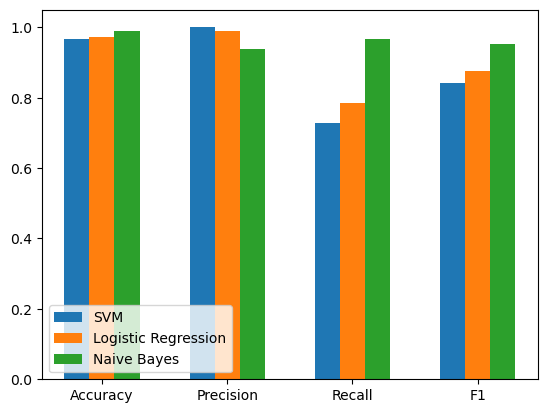
\includegraphics[width=\columnwidth]{images/image5.png}}
\caption{Comparison of results from each machine learning classification model.}
\end{center}
\vskip -.2in
\end{figure}

Upon analyzing the effectiveness of the classifiers we’ve chosen to run on our testing data, we see that typically the Naive Bayes classifier performs better than the SVM and Logistic Regression classifiers. The Naive Bayes classifier outperforms the other classifiers in accuracy, recall, and F1 score. The largest difference between the Naive Bayes model and the others we tested was in recall, where the Naive Bayes model had on average 27 less spam emails being classified as legitimate than the other algorithms. Despite the Naive Bayes classifier typically outperforming the other classifiers, all performed well on testing data, consistently scoring above at least 70\% across the board. 

The main concern we have with our current results is that of overfitting. The data set that we used to train and test our models was relatively small, having just over 5000 entries, so the models may have become too accustomed to the data set. If we were to redo the project, we would aim to test the model on more data in order to see if the conclusions we've reached are still valid on a larger scale.

\section{Summary}

Overall, the algorithms that we employed to detect spam emails were very effective for the data set we used. Other machine learning algorithms may also prove useful in this task, and would be enjoyable to test along with a larger data set.

\bibliography{spamML}
\bibliographystyle{icml2021}

\end{document}


% This document was modified from the file originally made available by
% Pat Langley and Andrea Danyluk for ICML-2K. This version was created
% by Iain Murray in 2018, and modified by Alexandre Bouchard in
% 2019 and 2021. Previous contributors include Dan Roy, Lise Getoor and Tobias
% Scheffer, which was slightly modified from the 2010 version by
% Thorsten Joachims & Johannes Fuernkranz, slightly modified from the
% 2009 version by Kiri Wagstaff and Sam Roweis's 2008 version, which is
% slightly modified from Prasad Tadepalli's 2007 version which is a
% lightly changed version of the previous year's version by Andrew
% Moore, which was in turn edited from those of Kristian Kersting and
% Codrina Lauth. Alex Smola contributed to the algorithmic style files.